% -*- latex -*-
%%%%%%%%%%%%%%%%%%%%%%%%%%%%%%%%%%%%%%%%%%%%%%%%%%%%%%%%%%%%%%%%
%%%%%%%%%%%%%%%%%%%%%%%%%%%%%%%%%%%%%%%%%%%%%%%%%%%%%%%%%%%%%%%%
%%%%
%%%% This text file is part of the source of 
%%%% `Parallel Computing'
%%%% by Victor Eijkhout, copyright 2012-2024
%%%%
%%%% ispux2024slides.tex : master file IXPUG presentation at SC2024
%%%%
%%%%%%%%%%%%%%%%%%%%%%%%%%%%%%%%%%%%%%%%%%%%%%%%%%%%%%%%%%%%%%%%
%%%%%%%%%%%%%%%%%%%%%%%%%%%%%%%%%%%%%%%%%%%%%%%%%%%%%%%%%%%%%%%%

\documentclass[10pt,t]{beamer}

\input courseformat

\usepackage{geometry,fancyhdr,wrapfig}
\usepackage{amssymb,amsmath,verbatim,graphicx,pslatex,multicol}
\usepackage{comment}
\newif\ifInBook \InBooktrue
\input book.inex
\input acromacs
\def\latexengine{}
%% \input bookmacs
%% \input articlemacs
%% \input ../../../scientific-computing-private/macros/commonmacs
%% \input idxmacs
%% \input idxpkgmacs
\input listingmacs
%% \input snippetmacs
\input ../../../scientific-computing-private/macros/tikzplot
\excludecomment{packt}

%% \lstset{
%%    keywordstyle=\usebeamercolor*[fg]{palette primary},
%%    commentstyle=\usebeamercolor*[fg]{palette secondary},
%%    stringstyle=\usebeamercolor*[fg]{palette tertiary}
%% }

%%\lstset{ keywordstyle=\usebeamercolor*[fg]{palette primary} }

\newcommand\codesnippetsdir{../snippets}
%% tikz graph customization
\def\graphwidth{.85}
\def\graphheight{.65}

%%
%% refer to sections in the HPC book
%%
\usepackage{xr-hyper}
% vol 1
\externaldocument[HPSC-]{scicompbook}

\def\qrcode{}
\begin{document}
\input lang

\author[Eijkhout]{Victor Eijkhout\\
  Texas Advanced Computing Center\\
  \texttt{eijkhout@tacc.utexas.edu}
}
\date{IxPUG2024@SC24}
%% \normalsize last formatted \today}
\title[C++ Parallel]{Modern C++ for Parallelism\\ in Scientific Computing}
\maketitle

\begin{frame}{Scientific computing parallelism}
  \begin{itemize}
  \item Large amounts of data: \\
    often cartesian multi-dimensional arrays, sometimes unstructured data
  \item Large amounts of parallelism:\\
    each element of output array independent.
  \item No explicit threading\\
    parallelism created by some runtime
  \item Range algorithm notion:\\
    do some operation on each element of a dataset
  \end{itemize}
\end{frame}

\begin{frame}[containsverbatim]{Power method}
  \hbox{}
  \begin{quote}
    \begin{tabbing}
      Let $A$ a matrix of interest\\
      Let $x$ be a random vector\\
      For \=iterations until convergence\\
      \> compute the product $y\leftarrow Ax$\\
      \> compute the norm $\gamma=\| y \|$\\
      \> normalize $x\leftarrow y/\gamma$\\
    \end{tabbing}
  \end{quote}
  \begin{itemize}
  \item Method for computing largest eigenvalue of a matrix
  \item Also Google Pagerank
  \item Stands for many scientific codes: Krylov methods, eigenvalues
  \end{itemize}
\end{frame}

\begin{frame}[containsverbatim]{Stencil operations}
  \hbox{}
  \vbox {\leavevmode \hsize=.8\textwidth
    \lower40pt\hbox{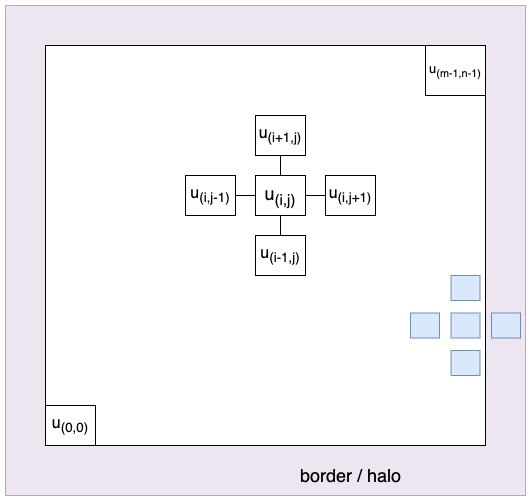
\includegraphics[scale=.22]{5pt_stencil_ij}}
    \hfill 
    \(
    \begin{array}{|r|r|r|}
      \hline
      \cdot&-1&\cdot\\
      \hline
      -1&4&-1\\
      \hline
      \cdot&-1&\cdot\\
      \hline
    \end{array}
    \)
    \hfill 
    }
  \begin{itemize}
  \item This rectangular $m\times n$ thing is the vector
  \item The $4,-1,\ldots$ stencil is~/ stands for the matrix.
  \item Goes by: difference stencil, convolution, Toeplitz matrix
  \end{itemize}
\end{frame}

\begin{frame}[containsverbatim]{Array parallelism}
  Traditional C implementation:
  
  \cxxverbatimsnippet{d2dscaleseq}
  \cxxverbatimsnippet{d2dseqindex}
  \begin{itemize}
  \item Two~/ three-dimensional loop
  \item all dimensions large
  \item every output element independent
  \end{itemize}
\end{frame}

\begin{frame}[containsverbatim]{Reductions}
  $\ell_2$ reduction:%
  \cxxverbatimsnippet{d2dnormseq}
  \begin{itemize}
  \item Parallel except for the accumulation
  \item Obviously should not be done through atomic operation
  \end{itemize}
\end{frame}

\begin{frame}[containsverbatim]{Stencil computation}
  Apply stencil to each $(i,j)$ index:
  \cxxverbatimsnippet{d2d5ptseq}
  \begin{itemize}
  \item Differential operator~/ image convolution
  \item Structure can be more complicated in scientific codes
  \end{itemize}
\end{frame}

\begin{frame}[containsverbatim]{Tools: \texttt{mdspan} and \texttt{cartesian\_product}}
  Data is declared as \lstinline{mdspan}:
  \begin{multicols}{2}
  \cxxverbatimsnippet{d2dspan0}
  \columnbreak
  \cxxverbatimsnippet{d2dspan2}
  \end{multicols}
  \cxxverbatimsnippet{d2dspan1}

  No performance loss~\cite{Hollman:mdspan}.
\end{frame}

\begin{frame}[containsverbatim]{\texttt{mdspan} and \texttt{cartesian\_product}}
  Index range is declared as \lstinline{range::views::cartesian_product}:
  \cxxverbatimsnippet{d2dinner}
  \begin{itemize}
  \item Vector allocated with size $(m+2b)\times(n+2b)$ to include border
  \item for handling of boundary conditions~/ halo regions in PDEs.
  \end{itemize}
\end{frame}

\begin{frame}[containsverbatim]{Implementation 1: OpenMP parallelism}
  Annotate loops as parallel and/or reduction:
  \cxxverbatimsnippet{d2dnormomp}
  \begin{itemize}
  \item Static assigment of iterations to threads by default
  \item Highly controlled affinity
  \item `\n{oned}' as above, `\n{clps}' for both loops collapsed
  \item Can be formulated as range algorithm.
  \end{itemize}
\end{frame}

\begin{frame}[containsverbatim]{Implementation 2: range over indices}
  Range-based for loop:
  \cxxverbatimsnippet{d2dnormspan}
  \begin{itemize}
  \item Range over indices, not over data
  \item Indices are a subset of the full data!
  \end{itemize}
\end{frame}

\begin{frame}[containsverbatim]{Stencil operation}
  Most complicated operation of the bunch:
\cxxverbatimsnippet{d2d5ptspan}
  \begin{itemize}
  \item Hard to formulate as range algorithm
  \item Performance not necessarily determined by floating point operations.
  \end{itemize}
\end{frame}

\begin{frame}[containsverbatim]{Implementation 3: Sycl}
  Open standard, but mostly pushed by Intel
  \cxxverbatimsnippet{syclbufaccess}
  \begin{itemize}
  \item Heterogeneous CPU/GPU code,\\
    transparent data movement
  \item Range algorithm-like syntax,\\
    but explicit task queue
  \end{itemize}
\end{frame}

\begin{frame}[containsverbatim]{Implementation 4: Kokkos}
  Open Source heterogeneous execution layer
  \cxxverbatimsnippet{kokkosbufaccess}
  \begin{itemize}
  \item Same code for CPU and GPU
  \item Implicit task queue
  \item Two-dimensional indexing
  \item Range algorithm-like philosophy
  \end{itemize}
\end{frame}

\begin{frame}[containsverbatim]{Comparing models (Intel)}
  \input d2dimodeltime

  Intel compiler. C-style variant fastest.
\end{frame}

\begin{frame}[containsverbatim]{Ratio to fastest (Intel)}
  \input d2dimodelratio
\end{frame}

\begin{frame}[containsverbatim]{Comparing models (Gcc)}
  \input d2dgmodeltime

  Gcc compiler. less variance between variants
\end{frame}

\begin{frame}[containsverbatim]{Ratio to fastest (Gcc)}
  \input d2dgmodelratio
\end{frame}

\begin{frame}[containsverbatim]{Where do we lose performance?}
  Hint: \n{perf} output on the `span' variant:
\begin{lstlisting}[language=verbatim]
    55.60%  [.] std::ranges::cartesian_product_view<std::ranges::iota_view<long, long>, std::ranges::iota_view<long, long> >::_Iterator<true>::operator+=
    18.73%  [.] __divti3
    11.33%  [.] linalg::bordered_array_span<float>::central_difference_from
     5.37%  [.] linalg::bordered_array_span<float>::scale_interior
     5.01%  [.] linalg::bordered_array_span<float>::l2norm
     2.69%  [.] __divti3@plt
\end{lstlisting}
Index calculations take lots of time.
\end{frame}

\begin{comment}
  \begin{frame}[containsverbatim]{Can we use execution policies?}
    \begin{itemize}
    \item Last time I tried there was a compiler issue
    \item That 5-point stencil is hard to express in range views!
    \end{itemize}
  \end{frame}
\end{comment}

\begin{frame}[containsverbatim]{Conclusion and Acknowledgement}
  \begin{itemize}
  \item `Fancy' schemes suffer from indexing overhead\\
    strongly implementation and compiler dependent.
  \item This work was supported by
    the Intel oneAPI Center of Excellence, and the 
    TACC STAR Scholars program,
    funded by generous gifts from TACC industry partners, including Intel, Shell, Exxon,
    and Chevron.\par
  \hbox to \textwidth{
    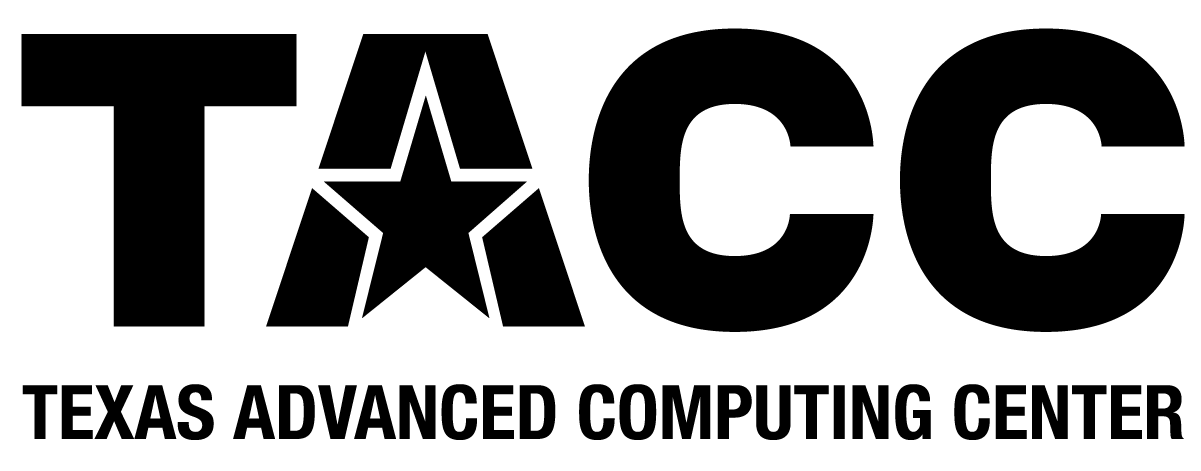
\includegraphics[scale=.4]{TACC-formal-Black-1c}
    \hfill
    \raise 5pt \hbox{
\includegraphics[scale=.12]{intel_cropped_t}}
    \hfill
    
\includegraphics[scale=.12]{STAR@4x}
    }
  \item Sycl code contributed by Yojan Chitkara
  \end{itemize}
\end{frame}

\begin{frame}{Bibliography}
  \bibliography{vle}
  \bibliographystyle{plain}
\end{frame}

\end{document}

\begin{frame}[containsverbatim]{}
  \begin{itemize}
  \item 
  \end{itemize}
\end{frame}

